\documentclass[10pt,a4paper]{article}
\usepackage[utf8]{inputenc}
\usepackage{amsmath}
\usepackage{amsfonts}
\usepackage{setspace}
\usepackage{amssymb}
\usepackage{graphicx}
\author{Brock Ellefson}
\title{CSCI432 HWN+1}
\begin{document}
\maketitle
\doublespacing

I've grown quiet a bit as a Computer Scientist this semester. In just this class alone, I've expanded my knowledge in this field tremendously. The majority of this has been in writing, during the beginning of the semester, I was a rather weak writer. When it comes to writing a proof, I think I have one major crux. I rush through it. Often times I have the concept correct, and show that I understand the problem being presented, however, I fail to fully express my thoughts and process of approaching the proof. Towards the beginning of the semester, I was getting frustrated whenever I got the proof correct but was getting docked points. I understand now that I was making proofs that were very elementary and vague. I would often forget to write out hypothesis and conclusions, even not defining new variables. After realizing these ?aws in my proofs, I've been trying to improve my formality. Its been a slow process but I believe I'm improving in comparison to the first few proofs we did in class. However, I think a strength I possess in academic writing is my step by step process to proving my proof. For example, in inductive proofs, I often for 1 get my conclusion and problem statement, but I always believed my inductive hypothesis and inductive steps where always pretty solid. For instance, this was the very first inductive proof I did for this class:
\\
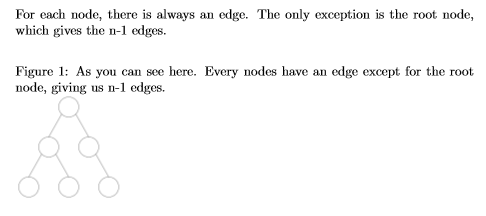
\includegraphics[scale=.75]{firstproof.png}

As compared to my most recent proof:
\\
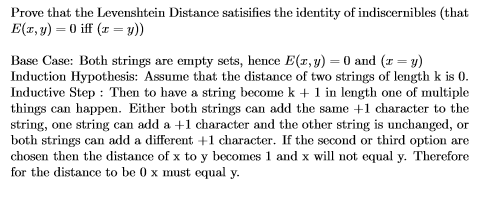
\includegraphics[scale=.75]{secondproof.png}

So I think it's clear that I have improved and grown when it comes to professional writing in Computer Science
\end{document}